% Santos. Supporting verification subsection.
\subsection{Compensated scan verification}\label{sec:additional-compensated-verification}
We validated the central point before the scan. The checks use the native IV stop, absence of amplitude rescalings, complex profile overlap, temporally unwrapped phase and consistent late-window fits. Both rates are given in reference speed over reference length. The selected spatial, velocity and timestep tests quantify sensitivity at two sampled points. The central half-step control with RKC2 retains the collision staging selected automatically by the nominal run. A companion RKC1 run measures staging sensitivity at the same smaller step. The nominal collisionless electron recurrence estimate is approximately 0.70 on the base grid. These are collisional simulations, and the late fit, profiles and velocity-grid comparison are used together to assess the observed mode.

\begin{center}\small
\begin{tabular}{@{}lrrrrr@{}}
\toprule
Control & $\Delta\widehat t$ & Native $\widehat\gamma$ & Native $\widehat\omega_r$ & Profile overlap & Wall (s)\\
\midrule
1.00: $n_z=32$ & 0.0009267 & 3.198 & +0.444 & 1.000000 & 248.3\\
1.00: half step, RKC1 & 0.0005437 & 3.204 & +0.444 & 1.000000 & 317.0\\
1.00: half step, RKC2 & 0.0005437 & 3.204 & +0.444 & 1.000000 & 335.8\\
2.00: $n_v=64$ & 0.0009362 & 3.948 & +0.596 & 1.000000 & 232.0\\
\bottomrule
\end{tabular}

\end{center}

\begin{figure}[H]\centering
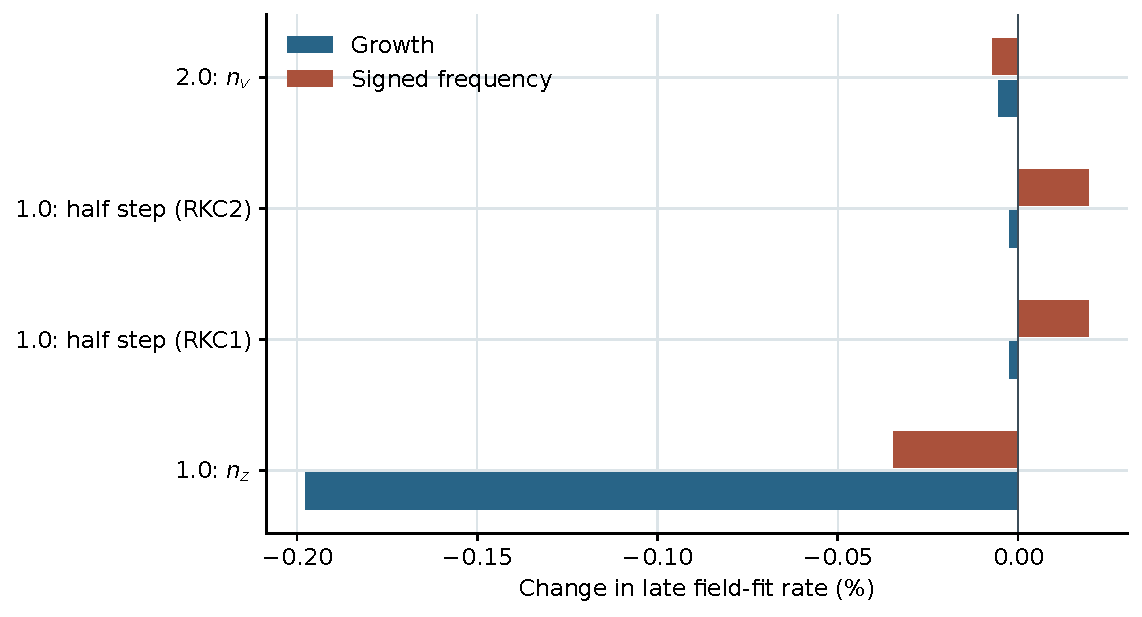
\includegraphics[width=.96\linewidth]{Figures/B_04_numerical_controls.pdf}
\caption{GENE rate sensitivity to targeted spatial, velocity and timestep checks, based on independent late complex-field fits. Contributor: Santos.}
\label{fig:additional-compensated-controls}
\end{figure}
